\begin{center}
    \renewcommand{\nextTitle}{ГЛАВА 4. ПРАКТЫЧНАЯ РЭАЛІЗАЦЫЯ}
    \addcontentsline{toc}{section}{\nextTitle}
    \section*{\nextTitle}
\end{center}

\vspace{5mm}

\renewcommand{\cursection}{4}
\setcounter{figure}{0}

\renewcommand{\nextTitle}{3.1 Распрацаванае праграмнае забеспячэнне}
\addcontentsline{toc}{subsection}{\nextTitle}
\subsection*{\nextTitle}

\vspace{5mm}

У якасці практычнай часткі, сярод іншага, было распрацаванае праграмнае забеспячэнне для правядзення рэканструкцыі
паверхні па наборы здымкаў і, пры наяўнасці, па дадатковых дадзеных, такіх як значэнні знешніх альбо ўнутраных
параметраў камер.

Праграма распрацоўвалася на C++, з выкарыстаннем бібліятэкаў Qt, OpenGL (для візуалізацыі
трохмерных мадэляў), TheiaSfm (\cite{theia-sfm}, змяшчае некаторыя алгарытмы камп'ютарнага зроку).
Праграмнае забеспячэнне даступнае для запуску на Ubuntu і macOS.

\vspace{3mm}

Базавы функцыянал уключае ў сябе:

\begin{itemize}
    \item працу з праектамі: стварэнне (прыклад на малюнку \cursection.\ref{fig:appa-new-project}),
    кіраванне, паўторнае адкрыццё, кіраванне пабудаванымі мадэлямі.
    \begin{figure}[H]
      \centering
      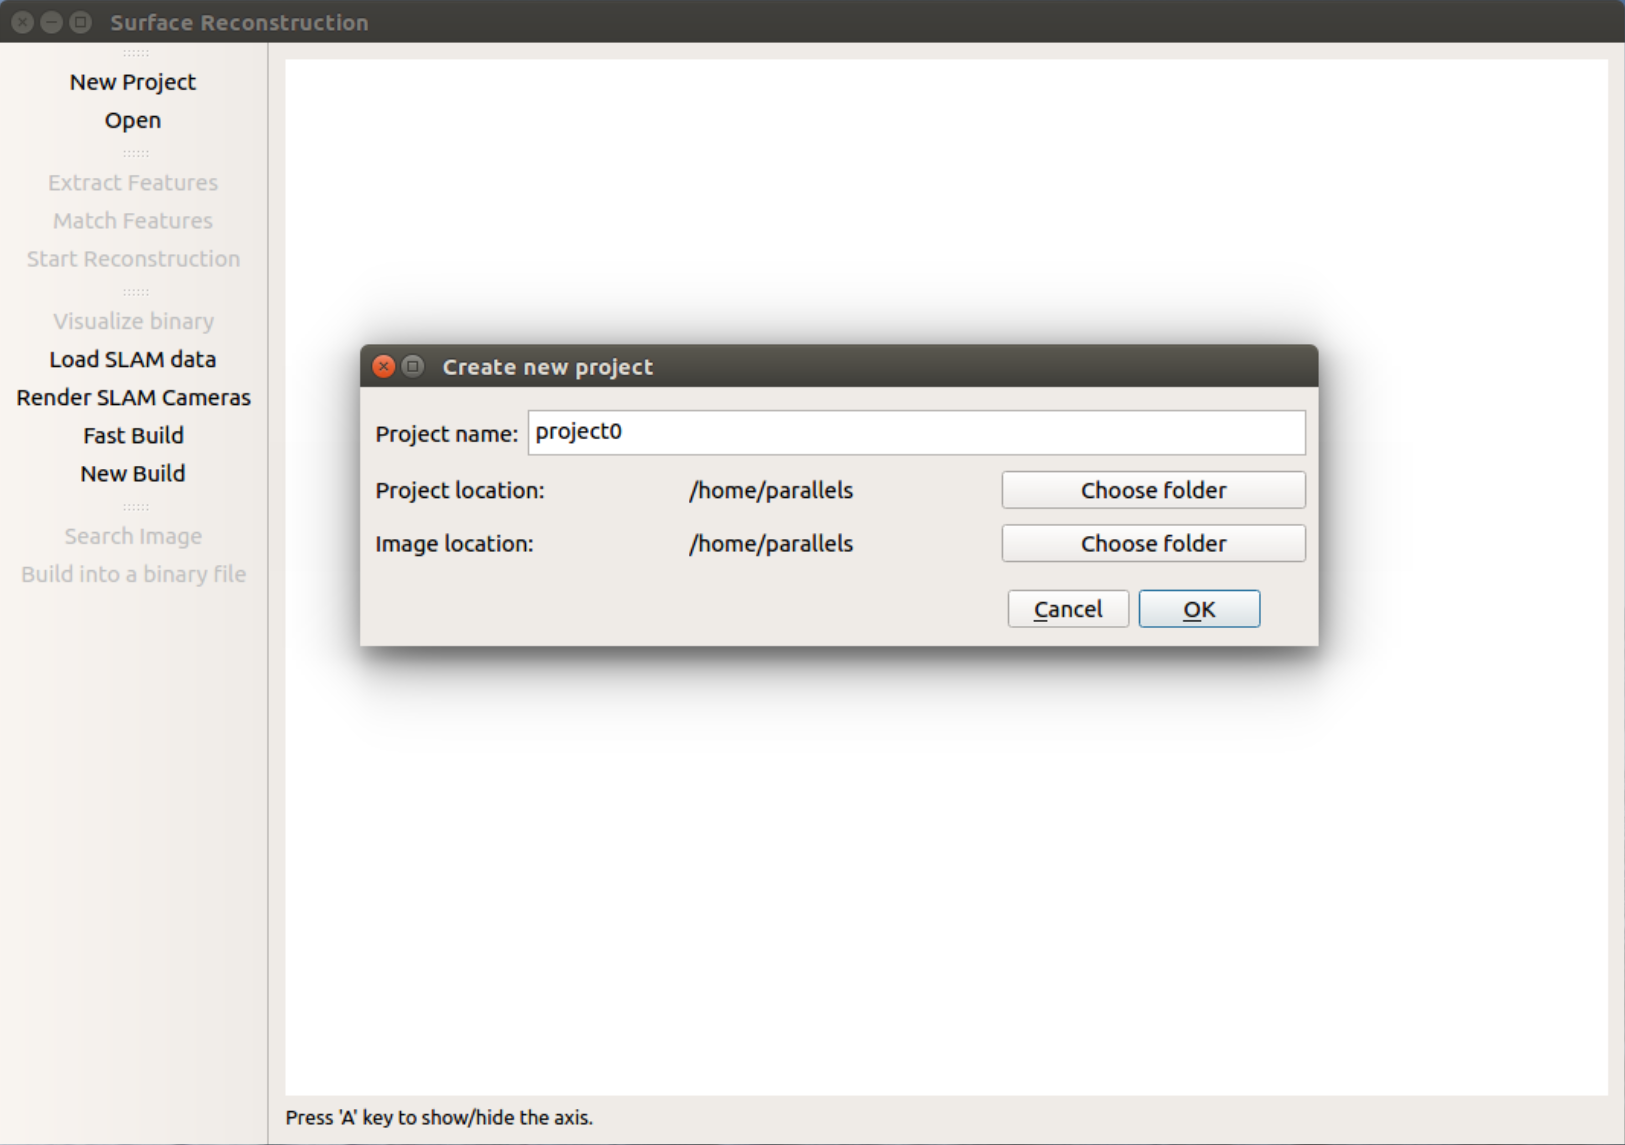
\includegraphics[width=\textwidth]{appa/new-project}
      \captionsetup{labelformat=empty}
      \caption{Малюнак \cursection.\arabic{figure}: стварэнне новага праекта}
      \label{fig:appa-new-project}
    \end{figure}
    \item выманне і апісанне ключавых кропак, захаванне іх у файлавую сістэму. Захаванне
    прамежкавых этапаў рэканструкцыі, такіх як апісаныя ключавыя кропкі, вельмі станоўча
    адбіваецца на часе запускаў на тых жа наборах дадзеных: замест паўторнага вымання кропак
    яны чытаюцца з файлавай сістэмы, тады як наступныя этапы могуць запускацца ўжо з іншымі параметрамі.
    \item падобны падыход і з пошукам адпаведнасцяў: знойдзеныя тым ці іншым спосабам адпаведнасці
    захоўваюцца ў файлавую сістэму для паўторнага выкарыстання.
    \item усе этапы рэканструкцыі кантралююцца вялікай колькасцю параметраў, асабліва
    зручна кіраваць якімі праз графічны інтэрфейс (як на малюнку \cursection.\ref{fig:appa-options}).
    \begin{figure}[H]
      \centering
      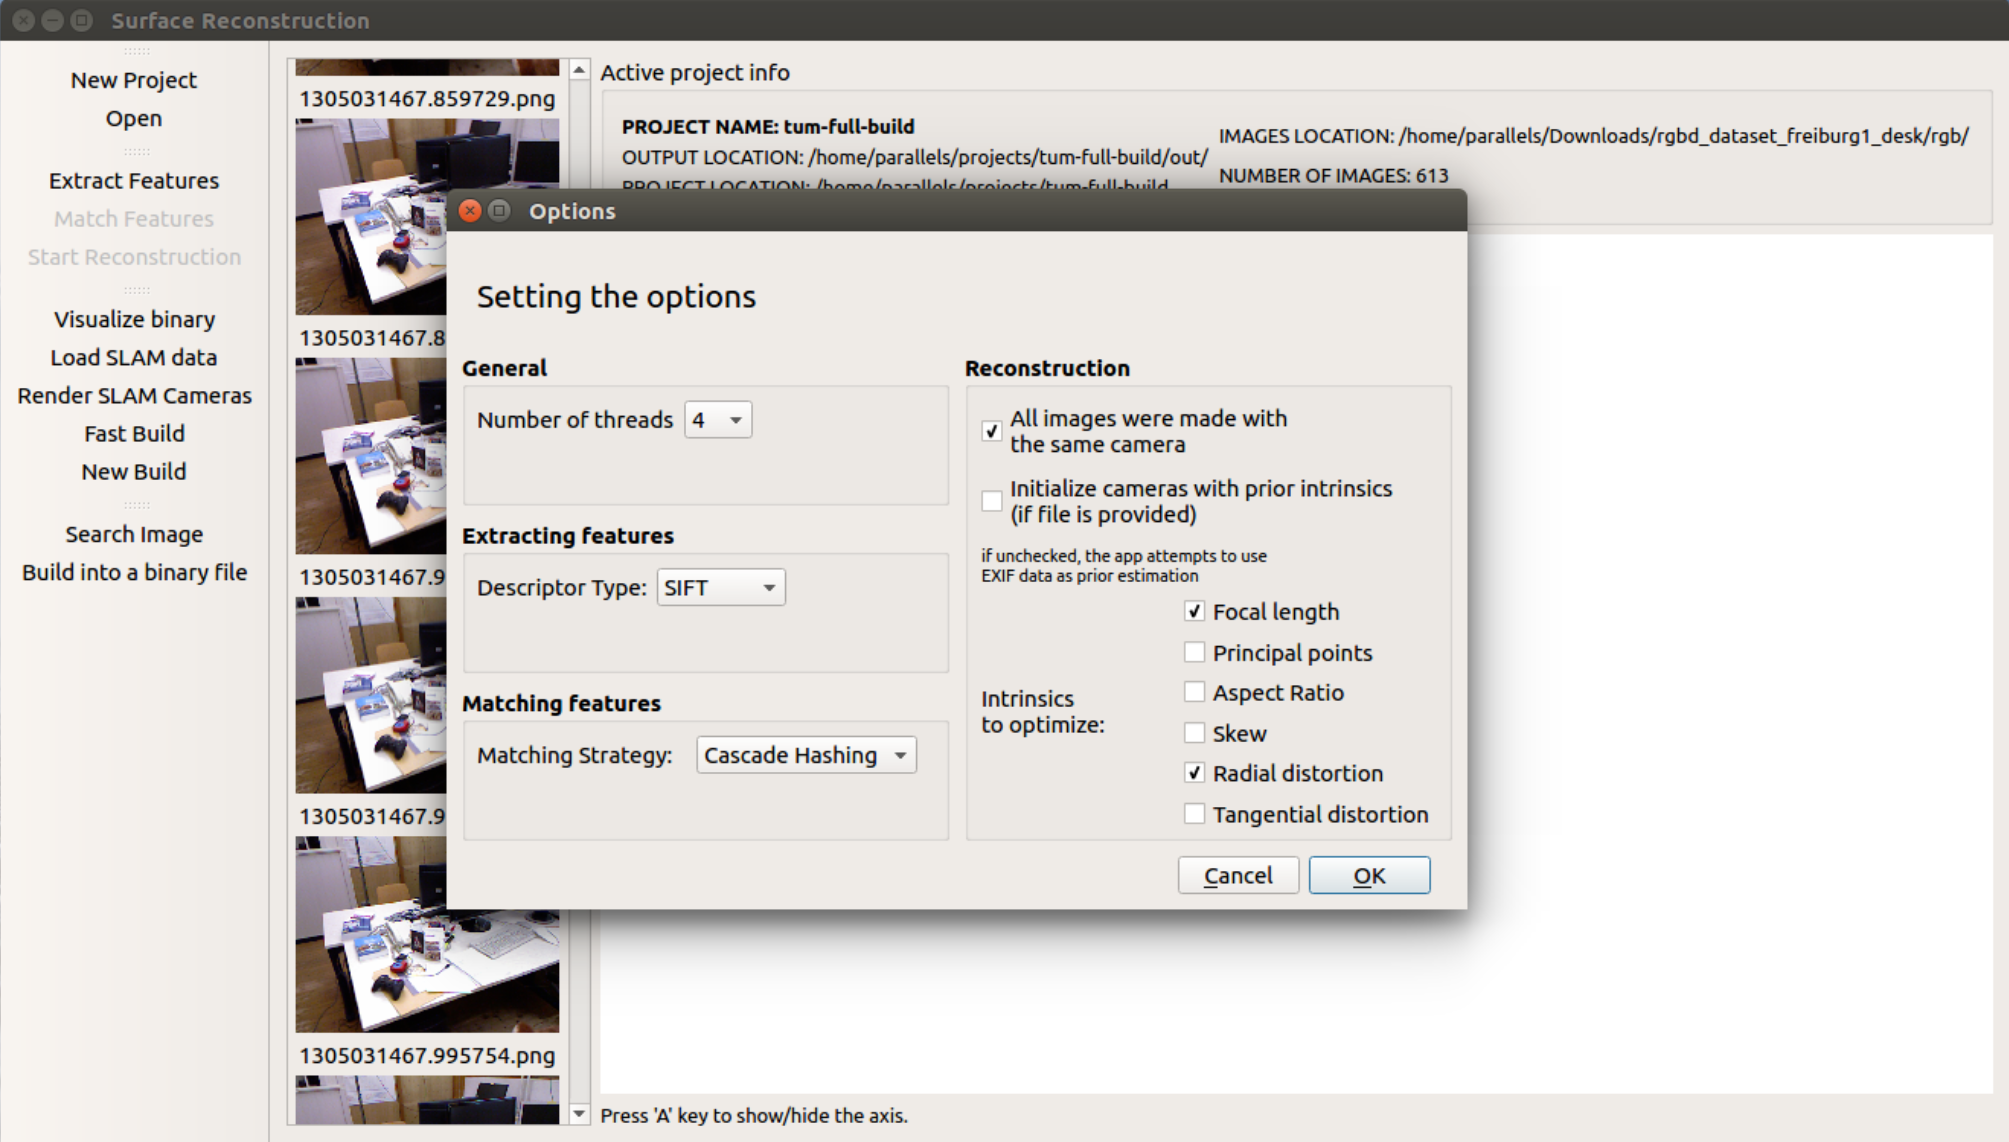
\includegraphics[width=\textwidth]{appa/options}
      \captionsetup{labelformat=empty}
      \caption{Малюнак \cursection.\arabic{figure}: налады, даступныя да зменаў пры запуску працэса рэканструкцыі}
      \label{fig:appa-options}
    \end{figure}
    \item наяўнасць рэжыма запуска праз камандны радок (малюнак \cursection.\ref{fig:appa-cli}),
    вельмі зручнага для частых запускаў і для напісання скрыптоў для правядзення эксперыментаў.
    Магчымасць праглядзець трохмерную мадэль прысутнічае пасля ў графічным інтэрфейсе.
    \begin{figure}[H]
      \centering
      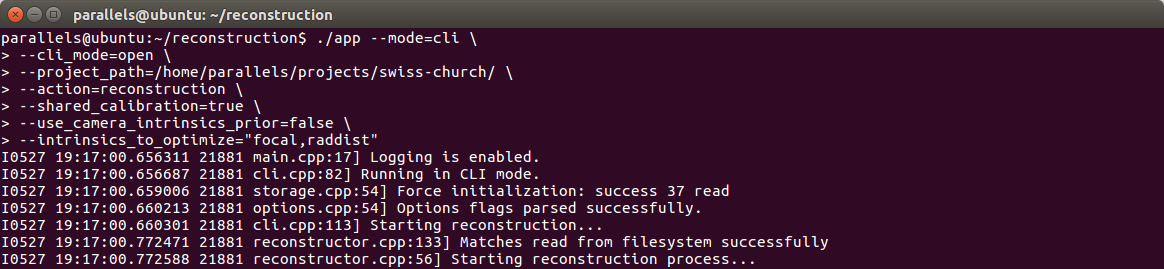
\includegraphics[width=\textwidth]{appa/cli}
      \captionsetup{labelformat=empty}
      \caption{Малюнак \cursection.\arabic{figure}: інтэрфейс каманднага радка}
      \label{fig:appa-cli}
    \end{figure}
    \item адна з асноўных функцыяў для якой, уласна, спатрэбілася распрацоўка графічнага інтэрфейса -
    акно візуалізацыі пабудаваных мадэляў. Прыклад праграмы з загружанай у памяць мадэллю можна
    пабачыць на малюнку \cursection.\ref{fig:appa-visual}.
    \begin{figure}[H]
      \centering
      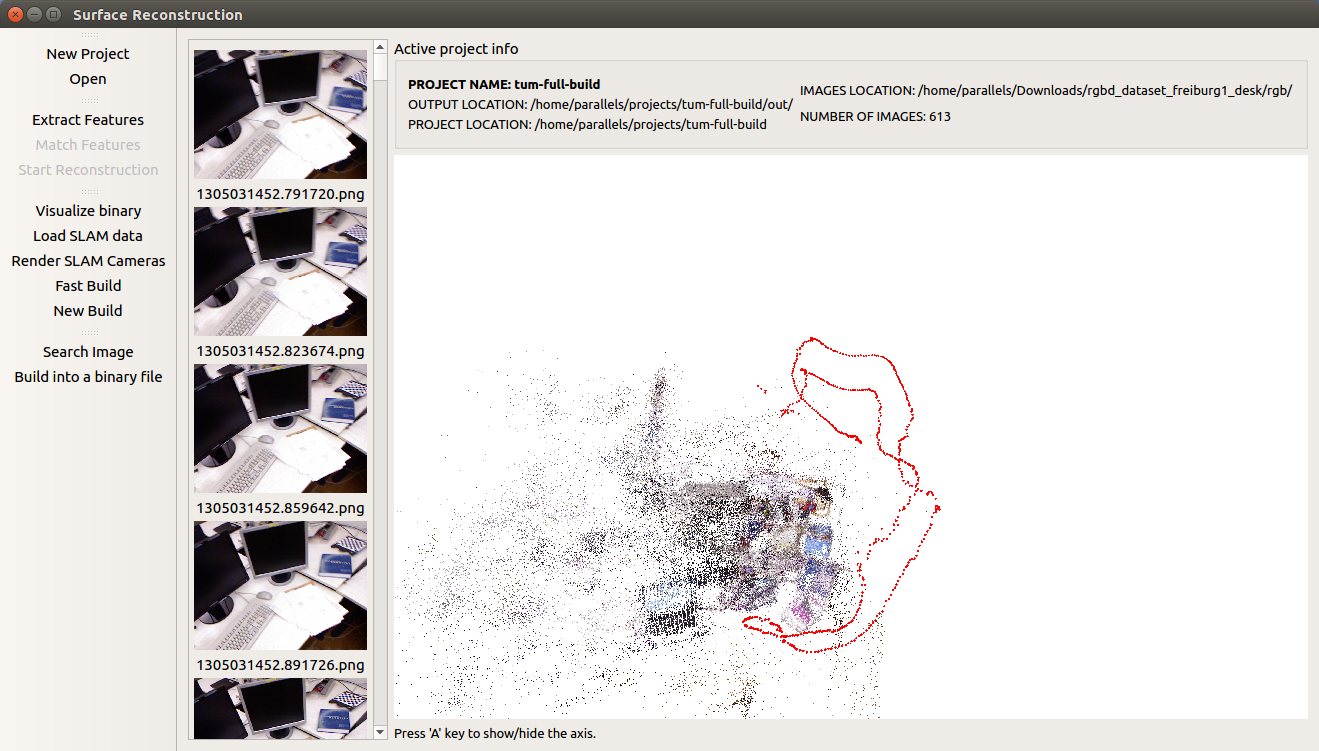
\includegraphics[width=\textwidth]{appa/visual}
      \captionsetup{labelformat=empty}
      \caption{Малюнак \cursection.\arabic{figure}: візуалізацыя воблака кропак ў рэжыме графічнага інтэрфейса}
      \label{fig:appa-visual}
    \end{figure}
    \item магчымасць націскаць выявы ў акенцы злева і падсвечваць адпаведныя ім камеры ў акне візуалізацыі.
    \item ініцыялізацыя унутраных параметраў камераў папярэднімі значэннямі.
    \item магчымасць працы ў рэжыме, калі кожная камера (з пункту гледжання алгарытмаў)
    з'яўляецца адной і той жа фізічнай камерай (для нашых задачаў мы амаль заўсёды працуем
    у гэтым рэжыме). Дадзены рэжым абагульняецца на выпадкі, калі, напрыклад,
    сярод усяго мноства здымкаў палова зроблена адной фізічнай камерай (з адным наборам
    унутраных параметраў), іншая палова - іншай камерай.
\end{itemize}

Важнай частка праграмы з'яўляецца інтэграцыя з SLAM-алгарытмамі: дадзеныя, якія падчас пралёту
генеруюць SLAM-сістэмы, захоўваюцца і пасля выкарыстоўваюцца ў праграме. Напрыклад, на малюнку
\cursection.\ref{fig:appa-slam-cameras} паказаныя адмаляваныя камеры, пазіцыі якіх
падлічаныя SLAM-алгарытмам. На жаль, некаторыя
з гэтых магчымасцяў толькі даступныя ў выглядзе прататыпаў і патрабуюць наступнай распрацоўкі.
Падрабязней пра распрацоўку сістэмы, якая б спалучала SLAM-алгарытм з традыцыйным алгарытмам
пабудовы мадэлі, распавядаецца ў наступным пункце.

\begin{figure}[H]
  \centering
  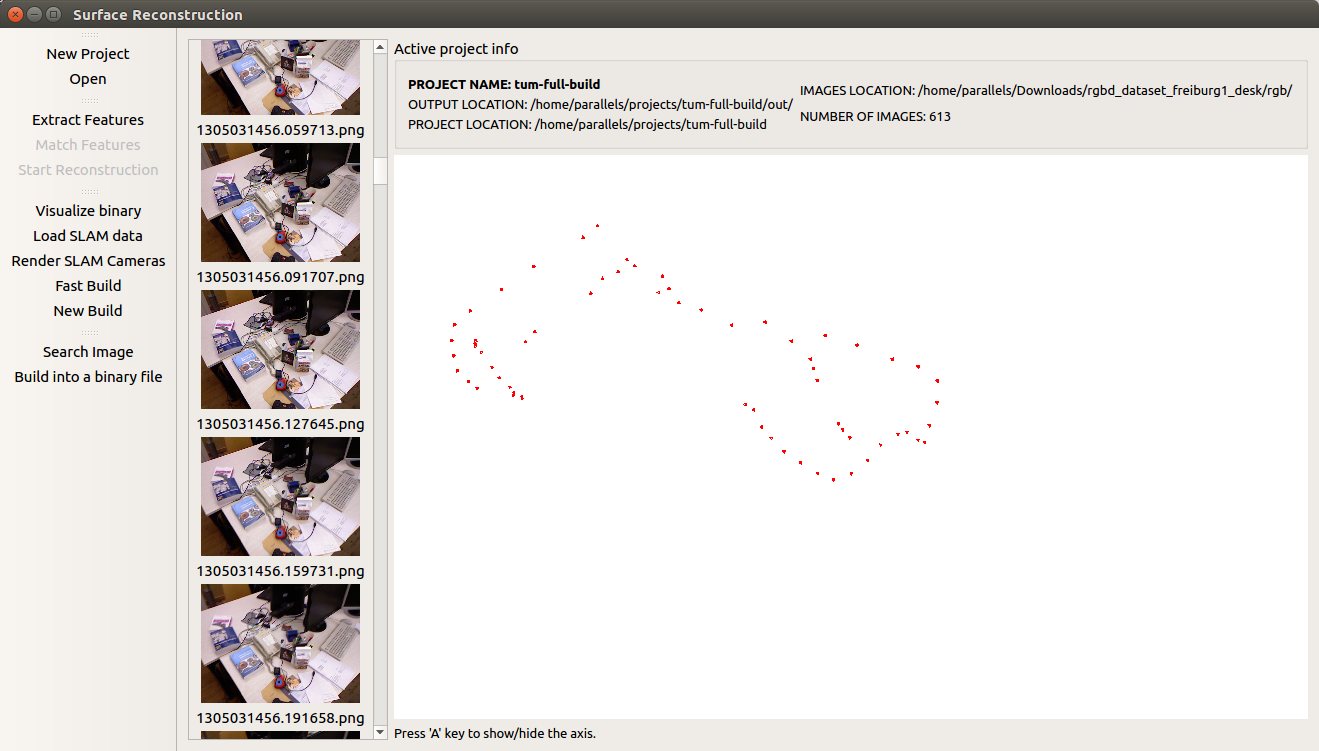
\includegraphics[width=\textwidth]{appa/slam-cameras}
  \captionsetup{labelformat=empty}
  \caption{Малюнак \cursection.\arabic{figure}: адмалёўка камераў, згенераваных SLAM-алгарытмам}
  \label{fig:appa-slam-cameras}
\end{figure}

\renewcommand{\nextTitle}{3.2 Інтэграцыя з SLAM-сістэмамі}
\addcontentsline{toc}{subsection}{\nextTitle}
\subsection*{\nextTitle}

\vspace{5mm}

Архітэктура сістэмы, рэалізацыяй якой я займаўся, і ўсе яе ключавыя вузлы схематычна
прадстаўленыя на малюнку \cursection.\ref{fig:architecture}.

Падрабязней будова сістэмы і яе кампанент, а таксама ўзаемадзеянне паміж яе часткамі
раскрываюцца ў наступных пунктах.

\begin{figure}[H]
  \centering
  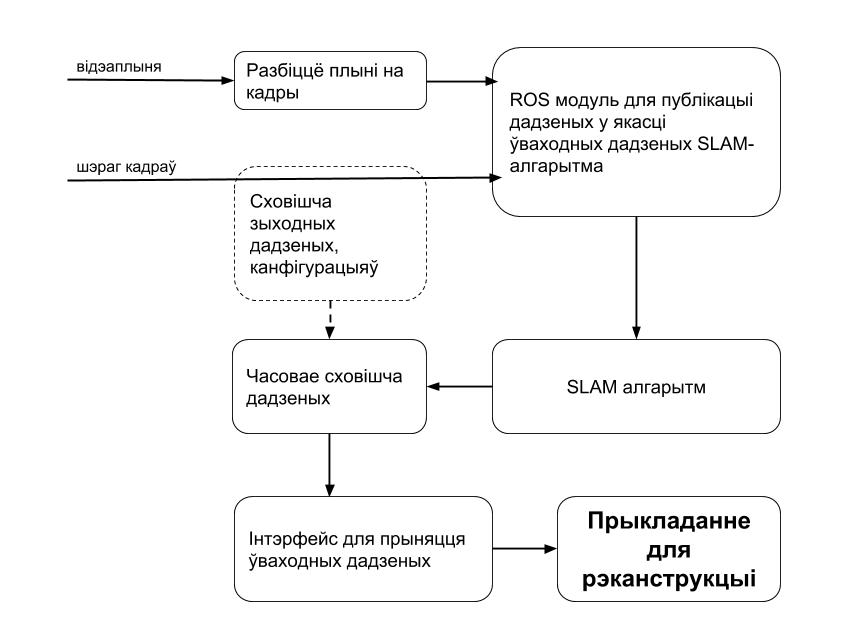
\includegraphics[width=.9\textwidth]{architecture}
  \captionsetup{labelformat=empty}
  \caption{Малюнак \cursection.\arabic{figure}: архітэктура спалучанай сістэмы}
  \label{fig:architecture}
\end{figure}

\renewcommand{\nextTitle}{3.2.1 ROS}
\addcontentsline{toc}{subsubsection}{\nextTitle}
\subsubsection*{\nextTitle}

ROS (The Robot Operating System) -- фрэймворк для напісання праграмнага забеспячэння
для робатаў, з'яўляецца наборам інструментаў, бібліятэкаў і
пагадненняў для зручнай і надзейнай працы з робатамі (\cite{288}). Патрэбнасць у фрэймворку ўзнікла
праз той факт, што стварэнне праграмнага забеспячэння для робатаў --
вельмі складаны і шматэтапны працэс; уніфікацыя спосабу камунікацыяў паміж часткамі вялікай
сістэмы дазваляе камандам працаваць над навігацыяй, рухам і зрокам робата асобна.

ROS пабудаваны на ідэі кліент-сервернага ўзаемадзеяння, што спрашчае працу ў размеркаваных
сістэмах, хаця і можа часам падавацца залішнім пры запуску на адной лакальнай машыне.

\vspace{4mm}

У аснове ROS ляжаць:

\begin{itemize}
  \item нізкаўзроўневы інтэрфейс перадачы паведамленняў,
  \item ананімная і асінхронная сістэма публікацыі і падпіскі на паведамленні,
  \item магчымасць рэалізацыі RPC для сінхроннага выкліку метадаў іншых пакетаў,
  \item глабальнае сховішча ключэй і значэнняў,
  \item зручныя сродкі дыягностыкі,
  \item інструменты для працы з ROS-ам праз графічны інтэрфейс: \textit{rviz}, \textit{rqt}.
\end{itemize}

Усе гэтыя ўласцівасці ROS-а робяць распрацоўку зручнай і лёгка ўбудоўваемай ў іншыя сістэмы.
Вялікая колькасць SLAM-алгарытмаў рэалізаваныя менавіта пад ROS і могуць не мець
уласных сродкаў візуалізацыі альбо ўводу дадзеных.

Казаць пра ROS можна не толькі у дачыненні да робатаў, але і, як у нашым выпадку, да
беспілотных лятальных апаратаў, бо разважанні не губляюць сваёй агульнасці. ROS зручны для працы
з любымі сістэмамі, неаўтаномнымі, паўаўтаномнымі альбо цалкам аўтаномнымі, якія ўключаюць у сябе
пэўны набор датчыкаў (такіх як камеры), маюць альбо не маюць уласных вылічальных магутнасцяў,
могуць кантраляваць сваё становішча ў прасторы. Пад такое азначэнне любы БПЛА, безумоўна, падыходзіць.

Падчас рэалізацыі ўласнага праграмнага забеспячэння мне давялося шчыльна пазнаёміцца з ROS-ам
і прынцыпамі арганізацыі працы ў гэтай аперацыйнай сістэме.

\renewcommand{\nextTitle}{3.2.2 Тыпы ўваходных інтэрфейсаў}
\addcontentsline{toc}{subsubsection}{\nextTitle}
\subsubsection*{\nextTitle}

У сістэме з малюнку \cursection.\ref{fig:architecture}
вялася праца з двума тыпамі ўваходных інтэрфейсаў для прыняцця дадзеных.

Першы -- перанакіраванне відэаплыні наўпрост з вэб-камеры ці любой іншай сістэмы захопу відэа.
У такім рэжыме мы найбольш набліжаемся да ўмоваў, якія можа сустрэць алгарытм пры запуску на
лятальным апараце пры выкананні рэальнага палёту. Прыблізна ў такім жа рэжыме працуе сапраўдны БПЛА
пры пралёце над мясцовасцю.

Другі -- публікацыя паслядоўнасці кадраў загадзя падрыхтаванага
набора дадзеных. Такі рэжым значна лепш падыходзіць для тэставання і адладкі алгарытмаў
і дае магчымасць паўтараць эксперыменты на аднолькавых дадзеных.

Падтрымка абодвух рэжымаў стала магчымай праз напісанне ўласных утылітаў для ROS
альбо мадыфікацыю існуючых. Трэба дадаць, што на наступных этапах мы працуем
з дадзенымі як з мноствам кадраў альбо выяваў -- такім чынам, пры наяўнасці відэаплыні
на ўваходзе ўзнікае патрэба ў разбіцці плыні на кадры з вызначанай частатой, захаванне кадраў
у форме асобнага датасэту, а таксама сінхранізацыя пазіцыяў камер з абранымі кадрамі з пачатковай
відэаплыні.

\renewcommand{\nextTitle}{3.2.3 Выманне дадатковых дадзеных са SLAM-алгарытмаў}
\addcontentsline{toc}{subsubsection}{\nextTitle}
\subsubsection*{\nextTitle}

Рэалізацыі большасці SLAM-алгарытмаў, разгледжаных у папярэдняй главе, даступныя ў вольным доступе
як праекты з адкрытым зыходным кодам. Аўтары каментуюць публікацыю як адначасова
унёсак у SLAM супольнасць і сродак для даследчыкаў з памежных галінаў \cite{murORB2}.

Распрацоўка ўласных SLAM-алгарытмаў не ставілася ў якасці мэты -- гэта вялікая праца,
якая патрабуе годы даследаванняў і, да таго ж, звычайна робіцца вялікай камандай распрацоўшчыкаў.
У гэтай працы выкарыстоўваюцца існуючыя SLAM рэалізацыі, удасканаленыя для нашых патрэбаў.

Адным з найбольш крытычных месцаў працы сістэмы з'яўляецца выманне ўсіх патрэбных нам дадзеных
са SLAM-алгарытмаў і узгадненне гэтага фармату дадзеных, для паспяховага пераходу да
наступных крокаў.

Першае, што варта тут згадаць -- патрэбныя нам дадзеныя не выдаюцца алгарытмамі ў гатовым выглядзе.
Цікавыя нам значэнні параметраў схаваныя ўнутры рэалізацыяў, але праз наяўнасць адкрытага зыходнага
кода з'яўляецца шанец працаваць з патрэбнымі нам дадзенымі.
У якасці выходных дадзеных нас найбольш цікавіць граф узаемабачнасці кропак з камераў
(\textit{covisibility graph}) -- граф, вяршынямі якога з'ўляюцца камеры (альбо ключавыя кадры), рэбры
праводзяцца паміж тымі вяршынямі, адпаведныя камеры якіх маюць дастаткова вялікую агульную
аглядаемую прастору (вымяраецца ў колькасці знойдзеных агульных трохмерных кропак). Таксама
цікаўнасць прадстаўляюць ацэнкі пазіцыяў камер, якія можна альбо прыняць за ісціну, альбо
скарыстаць у якасці апрыорнай ацэнкі. Патрэба ва ўсіх гэтых дадзеных прымушае нас
разбіраць той ці іншы SLAM-алгарытм на кавалкі, шукаць патрэбныя дадзеныя у кодзе і знаходзіць магчымасці
выгрузкі іх у вонкавую прастору.

Па-другое, працуючы з рознымі SLAM-алгарытмамі, мы павінны падыходзіць да кожнага з іх
індывідуальна, шукаючы магчымасць выгрузіць патрэбныя нам дадзеныя, але ў выніку,
прадставіць дадзеныя ва ўніфікаванай форме, незалежнай ад выкарыстанага SLAM-алгарытма.
Індывідуальная праца з кожным асобна ўзятым алгарытмам моцна ўскладняе нашую задачу.

У выніку, большасць часу была прысвечаная ORB-SLAM (\cite{murTRO2015}, \cite{murORB2}) як сістэме,
якая давала найбольш надзейныя вынікі для ацэнак пазіцыяў камер, а таксама якая
досыць зручна інтэгравалася у архітэктуру з малюнку \cursection.\ref{fig:architecture}.

\renewcommand{\nextTitle}{3.2.4 Аптымізацыя камунікацыяў з дапамогай ROS}
\addcontentsline{toc}{subsubsection}{\nextTitle}
\subsubsection*{\nextTitle}

Яшчэ адным накірункам працы з'яўлялася аптымізацыя камунікацыяў паміж часткамі сістэмы.
У некаторых месцах дадзеныя ў кодзе перадаюцца праз файлавую сістэму, але ў большасці
сітуацыяў камунікацыі аптымізаваныя з дапамогай убудаваных сродкаў ROS: публікацыя ў ROS-аўскі
``topic'' з аднаго боку і праслухоўванне з іншага з'яўляецца, у агульным
выпадку, значна больш дасканалым спосабам злучэння асобных элементаў сістэмы з малюнку \cursection.\ref{fig:architecture}
у адно суцэльнае. Гэты спосаб таксама дазваляе павялічыць хуткасць камунікацыяў,
бо абмен дадзенымі ідзе праз RAM-памяць замест файлавай сістэмы.

\renewcommand{\nextTitle}{3.2.5 Статус распрацаванасці}
\addcontentsline{toc}{subsubsection}{\nextTitle}
\subsubsection*{\nextTitle}

Была рэалізаваная большасць кампанентаў сістэмы, пазначаных на схеме \cursection.\ref{fig:architecture},
але праз той факт, што для ўзгодненай працы ўсёй сістэмы патрэбная яе поўная рэалізацыя,
патрэбнае правядзенні серыі інтэграцыйных тэстаў і серыі дадатковых эксперыментаў, сістэма не была сапраўды
даведзеная да кропкі, на якой з'явілася б магчымасць падзяліцца вынікамі, якія б сцвярджалі, наколькі жыццяздольнай
з'яўляецца падобная архітэктура. У любым выпадку, ёсць упэўненасць, што паколькі запуск SLAM-алгарытма
з'яўляецца ``бясплатным'' -- у тым сэнсе, што адбываецца ў рэальным часе і затрачвае толькі вылічальныя
магутнасці сістэмы, але не часавыя, то інтэграцыя SLAM-сістэмаў з традыцыйнымі будзе мець станоўчы
эфект і пазітыўна адлюструецца на колькасных і якасных характарыстыках рашэння задачы рэканструкцыі паверхні.

\newpage
